\section{System Design}
The Power Information Collection Architecture (PICA) is a collection of components whose purpose is to accurately collect and relate information about power quality and consumption to a consumer. Designed to be modular, these components can operate individually or together as a suite of sensors and controls to empower the consumer with more accurate and up-to-date information about power usage. The four major systems seen in figure \ref{fig:sys_overview} compose the PICA system.

\begin{figure}[htbp]
\begin{center}
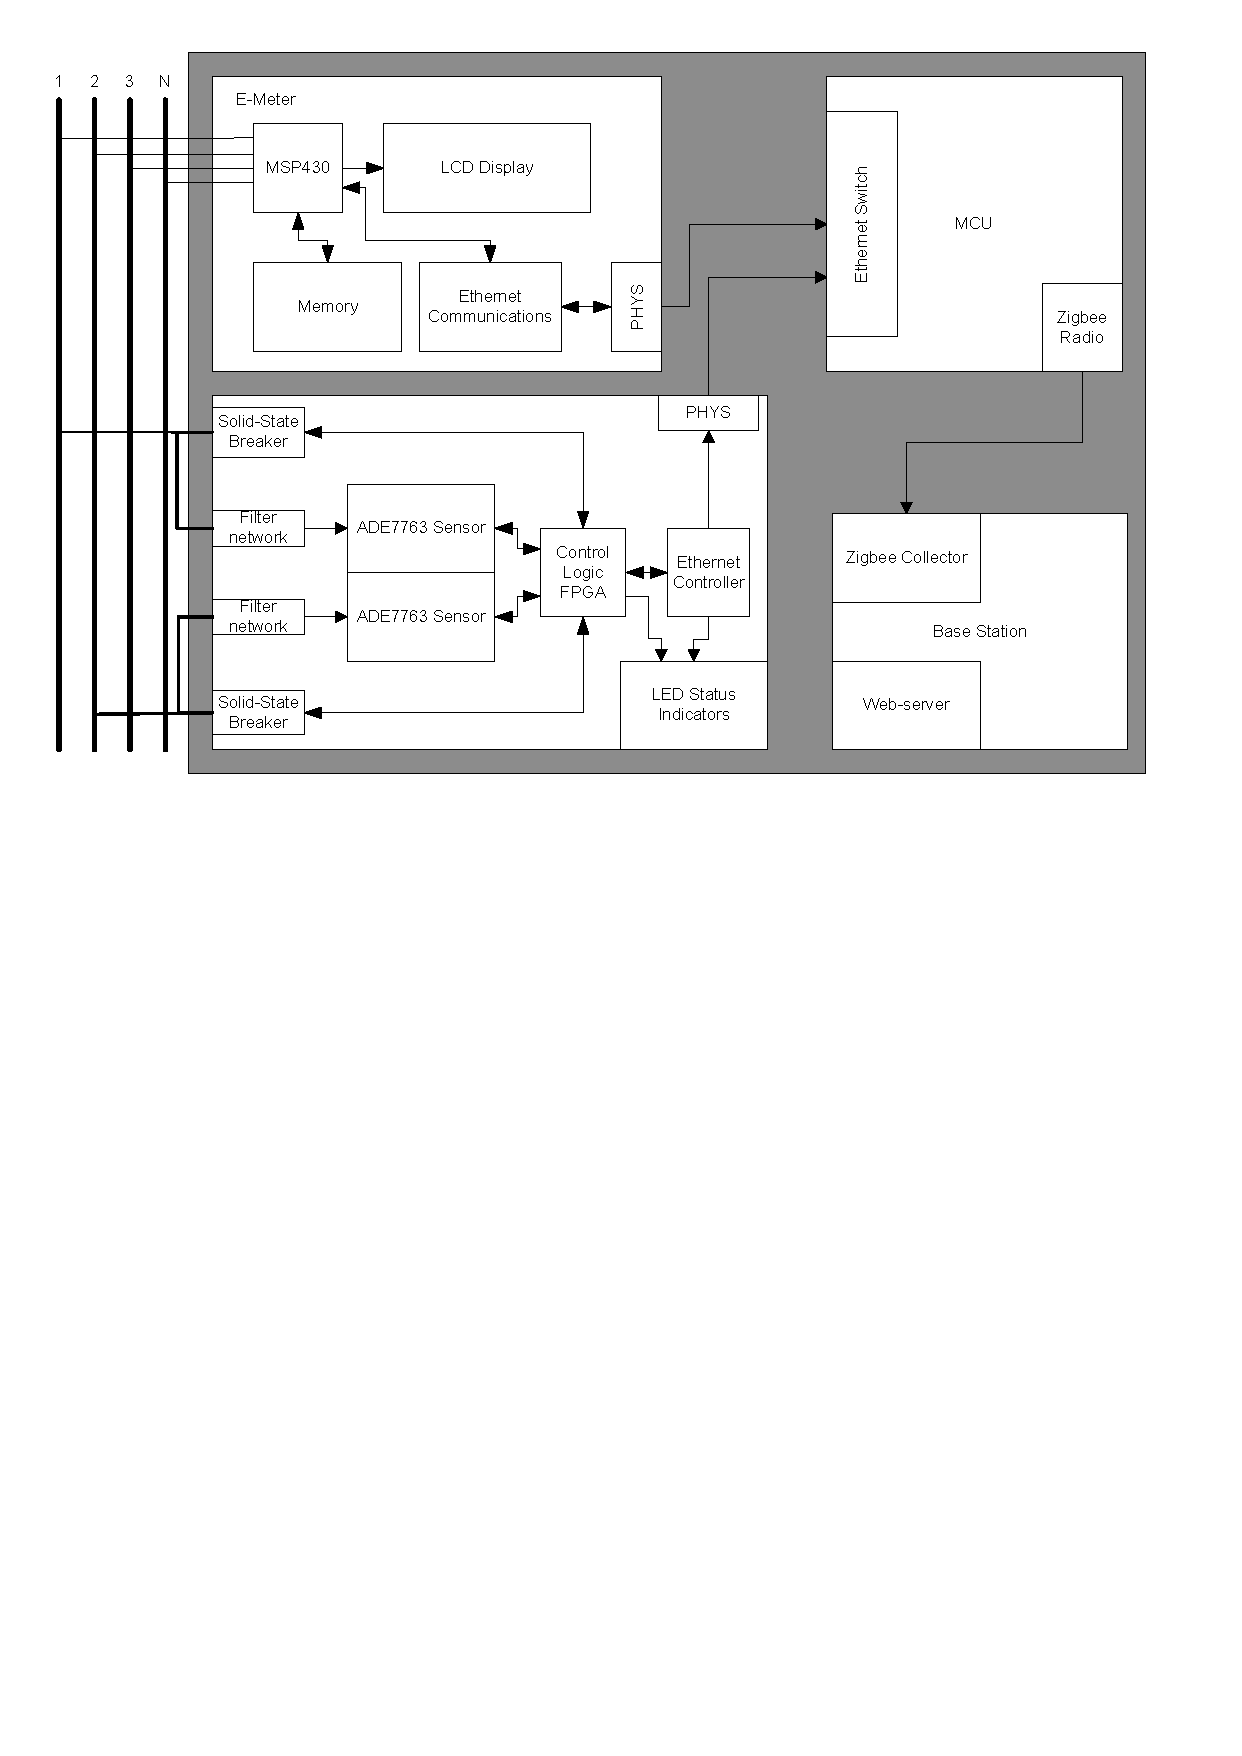
\includegraphics[width=5in]{figures/System_Diagram}
\caption[System Overview]{An overview of the 4 major systems of the PICA system.}
\label{fig:sys_overview}
\end{center}
\end{figure}


The E-Meter is a smart metering device; capable of monitoring single or multi phase power installations, this device replaces the current �dumb� meter that exists on the exterior of most residential and commercial buildings. The E-Meter monitors how much power an entire installation (e.g. a home or business) consumes over a given period. The power company collects this information and uses it for billing purposes. By introducing a smarter power meter, Team PICA can monitor reactive power, flicker voltage, phase angle, frequency, and, peak voltage in addition to total power consumption. Once collected, the power company can use this information to understand the health and status of the electric grid more completely. A web interface then provides the consumer with an hour-by-hour overview of their power consumption. The E-Meter provides an LCD display on the outside to display the instantaneous power usage in kilowatt-hours.

The smart breaker is a solid-state replacement for the traditional electromechanical breaker found in electric panels. Using MOSFET technology to mimic a fault-interrupter, these solid-state breakers can sense a fault in the circuit and respond in a fraction of the time it takes traditional breakers to trip. Each breaker includes status lights to indicate the status of the circuit (on, off, fault), and a sensor to provide circuit level information on power usage. A system on a chip (SoC) collects the information provided by the sensors and uses the instantaneous measurements to control the breakers before packaging and shipping the data to the system controller for transmission to the MCU. 

The master control unit (MCU) controls the transmission of data to the PICA base station over the Zigbee 802.15 radio link. The MCU acts as a buffer and arbitrator for the Zigbee radio and receives data in TCP/IP packages from each subsystem. Onboard, the MCU stores packages until the mesh-network comes up and then transmits packages until its buffers are empty. The prototype MCU comes from a WRT54G wireless router produced by Cisco sold under the name Linksys and targeted at the home networking market.

The PICA base station collects all the sensor data, collates the data, and hosts a webpage where it displays the information. The consumer can access the webpage by attaching the PICA base station to a network router or directly to the network interface card (NIC) of a personal computer. The PICA base station acts as the collector node for the Zigbee mesh network. The base station could provide a control point for future smart devices in the home, such as a thermostat or other smart appliances. The base station connects to an in-home display that displays usage information.
